\documentclass[14pt, a4paper]{report}
\usepackage[utf8]{inputenc}
\usepackage[russian]{babel}
\usepackage{multirow}
\usepackage{graphicx}
\usepackage{slashbox}
\renewcommand{\thesection}{\arabic{section}.}
\title{\textbf{Отчет о выполнении лабораторной работы 2.1.6 "Эффект Джоуля–Томсона"}}
\author{Калашников Михаил, Б03-205}
\date{}

\begin{document}

\maketitle

\textbf{Цель работы:} 1) определение изменения температуры углекислого газа при протекании через малопроницаемую перегородку при разных начальных значениях давления и температуры; 2) вычисление по результатам опытов коэффициентов Ван-дер-Ваальса ''$a$'' и ''$b$''.  

\textbf{Оборудование:} 
\begin{itemize}
  \item трубка с пористой перегородкой;
  \item  труба Дьюара;
  \item термостат ($\sigma_T=0,01\ K$);
  \item дифференциальная термопара;
  \item микровольтметр ($\sigma_U=1\ \mu V$)
  \item балластный баллон;
  \item манометр ($\sigma_{\Delta P}=0.1\ atm$).
\end{itemize}

\section{Теоретическая часть}

Эффектом Джоуля–Томсона называется изменение температуры газа, медленно протекающего из области высокого в область низкого давления в условиях хорошей тепловой изоляции. Изменение характеризуется коэффициентом Джоуля-Томсона:
\[\mu=\frac{\Delta T}{\Delta P}=\frac{(2a/RT)-b}{C_p}\]

Температура, при которой коэффициент меняет знак называется температурой инверсии, и, используя связь между коэффициентами $a$ и $b$ и критической температурой, получим:
\[T_{inv}=\frac{27}{4}T_{cr}\]

\section{Экспериментальная установка}

Схема установки для исследования эффекта Джоуля–Томсона в углекислом газе представлена на рисунке. Основным элементом установки является трубка 1 с пористой перегородкой 2, через которую пропускается исследуемый газ. Углекислый газ под повышенным давлением поступает в трубку через змеевик 5 из балластного баллона 6. Давление газа в трубке измеряется манометром М и регулируется вентилем В. Разность температур газа до перегородки и после нее измеряется
дифференциальной термопарой медь -- константан. Константановая проволока соединяет спаи 8 и 9, а медные проволоки подсоединены к цифровому вольтметру 7.  Для уменьшения теплоотвода трубка с пористой перегородкой помещена в трубу Дьюара 3, стенки которой посеребрены, для уменьшения теплоотдачи, связанной с излучением. Для уменьшения теплоотдачи за счет конвекции один конец трубы Дьюара уплотнен кольцом 4, а другой закрыт пробкой 10 из пенопласта. Такая пробка практически не создает перепада давлений между внутренней полостью
трубы и атмосферой.

\begin{figure}[!ht]
\centering
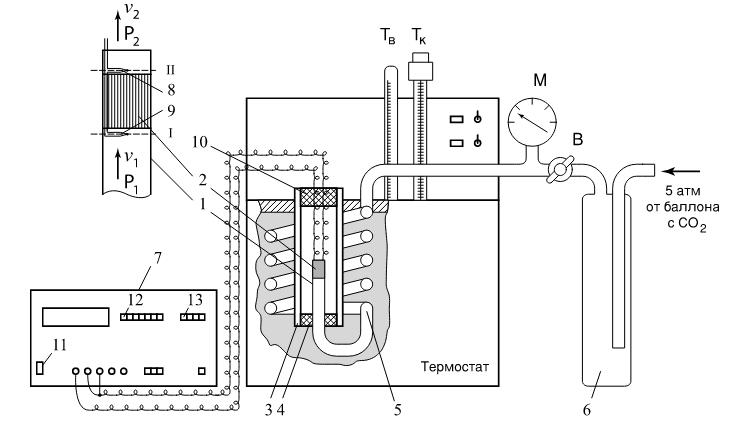
\includegraphics[scale=0.6]{terma_1_1.png}
\label{image1}
\caption{Схема установки для изучения эффекта Джоуля–Томсона}
\end{figure}

\section{Проведение эксперимента}

\begin{enumerate}
\item Убедившись в работспособности экспериментальной установки, можем приступить к выполнению измерений.
\item Включим термостат и выставим комнатную температуру в 20 градусов Цельсия.
\item Зафиксируем значение вольтметра при отсутствии перепада давления.
\[U_0=-5\ \mu V\]
Откроем вентиль В настолько, чтобы перепад давлений составил 4 атмосферы.
\item Выждав время, достаточное для окончания переходных процессов, зафиксируем значение вольтметра в таблицу 1.
\item Понизив давление на полатмосферы и снова выждав некоторое время, запишем показания вольтметра.
\item Повторим предыдущий пункт понижая давление вплоть до 2 атмосфер.
\item Повысим температуру термостата и повторим предыдущие пункты.

\end{enumerate}

\section{Обработка данных}

\begin{enumerate}
\setcounter{enumi}{7}

\item Используя табличные значения зависимости напряжения на термопаре от разности температуры на термопаре (таблица 2), переконвертируем значения таблицы 1 по формуле:
\[\Delta T=\frac{1}{\alpha(T)}(U-U_0)\]
Полученный результат отобразим в таблице 3.

\item Отложим полученные точки на графике $\Delta T (\Delta P)$. По наклону графика получим коэффициент Джоуля-Томсона для каждой температуре (таблица 3).

\item Мы знаем, что зависимость $\mu(\frac{1}{T})$ линейна и представима в виде
\[\mu(T)=\frac{2a}{RC_p}\frac{1}{T}-\frac{b}{C_p}\]
Проведем прямую $y=kx+m$ через значения $\mu$ и $\frac{1}{T}$, полученные в ходе эксперимента. Из параметров этой прямой можно найти коэффициенты $a$ и $b$:
\[a=\frac{kRC_p}{2};\quad b=-C_pm\]
Из справочника, для углекислого газа $C_p=41\ \frac{J}{mol\cdot K}$.
Температуру инверсии найдем по формуле:
\[T_{inv}=\frac{2a}{Rb}\]


\end{enumerate}

\section{Расчет погрешностей}

Относительная случайная погрешность коэффициента $a$ равна относительной погрешности коэффициента наклона прямой $\mu(\frac{1}{T})$. Последняя так же определяется из метода наименьших квадратов. Аналогично можно найти отнгосительную случайную погрешность коэффициента $b$.
\[\varepsilon_{a(rand)}=\varepsilon_k=\frac{\sigma_k}{k}=9.1\%\]
\[\varepsilon_{b(rand)}=\varepsilon_m=\frac{\sigma_m}{m}=11.0\%\]

Приборную погрешность найдем из формулы погрешности косвенных измерений.
\[\varepsilon_{a(inst)}=\sqrt{\varepsilon_T^2+\varepsilon_{\Delta T}^2+\varepsilon_{\Delta P}^2}=4.0\%\]
\[\varepsilon_{b(inst)}=\sqrt{\varepsilon_{\Delta T}^2+\varepsilon_{\Delta P}^2}=4.0\%\]
\[\varepsilon_{\Delta T}=\varepsilon_U=\sigma_U<\frac{1}{U-U_0}>,\quad \varepsilon_T=\sigma_T<\frac{1}{T}>, \quad \varepsilon_P=\sigma_P<\frac{1}{P}>\]

Полная погрешность равна:
\[\varepsilon_a=\sqrt{\varepsilon_{a(rand)}^2+\varepsilon_{a(inst)}^2}=9.9\%\]
\[\varepsilon_b=\sqrt{\varepsilon_{b(rand)}^2+\varepsilon_{b(inst)}^2}=11.7\%\]

Таким образом, величины $a$ и $b$ равны:
\[a=1.9\pm0.2\ \frac{Pa\cdot m^6}{mol^2} \quad b=(1.3\pm0.1)\cdot10^{-3}\ \frac{m^3}{mol}\]

Найдем температуру инверсии:
\[T_{inv}=\frac{2a}{Rb}=372\pm57\ K\]

\section{Вывод}

Полученные значения очень сильно отличаются от табличных значений. Коэффициент $a$ превышает в 5 раз, $b$ -- в 30 раз. Температура инверсии в 6 раз больше табличного значения. Очевидно, точности уравения Ван-дер-Ваальса недостаточно при обработки результатов данного эксперимента.

\section{Приложения}

\begin{table}[!ht]
\centering
\begin{tabular}{| c | c | c | c | c | c |}
\hline
\backslashbox{$t, ^\circ C$}{$\Delta P,\ atm$} & $4,0$ & $3,5$ & $3,0$ & $2,4$ & $2,0$ \\
\hline
20,00	& 91	& 71	& 53	& 34	& 21 \\
\hline
25,00	& 88	& 69	& 53	& 38	& 28 \\
\hline
35,00	& 87	& 74	& 62	& 44	& 32 \\
\hline
45,00	& 81	& 72	& 61	& 47	& 38 \\
\hline
55,00	& 72	& 68	& 59	& 45	& 37 \\
\hline
\end{tabular}
\label{table1}
\caption{Показания вольметра в $\mu V$ в зависимости от перепада давления $\Delta P$ и температуры термостата $T$}
\end{table}

\begin{table}[!ht]
\centering
\begin{tabular}{| c | c | c | c | c | c |}
\hline
$t, ^\circ C$ &		20 &	25 &	35 &	45 &	55 \\
\hline
$\alpha, \mu V/K$ &	40,3 &	40,7 &	41,6 &	42,5 &	43,3 \\
\hline
\end{tabular}
\label{table2}
\caption{Зависимость чувствительности термопары от температуры}
\end{table}

\begin{table}[!ht]
\centering
\begin{tabular}{| c | c | c | c | c | c |}
\hline
\backslashbox{$T, K$}{$\Delta P,\ kPa$} & $410$ & $350$ & $300$ & $240$ & $200$ \\
\hline
293,15	& 2,39	& 1,89	& 1,44	& 0,97	& 0,65 \\
\hline
298,15	& 2,29	& 1,82	& 1,43	& 1,06	& 0,81 \\
\hline
308,15	& 2,21	& 1,90	& 1,61	& 1,18	& 0,89 \\
\hline
318,15	& 2,02	& 1,81	& 1,55	& 1,22	& 1,01 \\
\hline
328,15	& 1,78	& 1,69	& 1,48	& 1,15	& 0,97 \\
\hline
\end{tabular}
\label{table3}
\caption{Перепад температуры $\Delta T, K$ в зависимости от перепада давления $\Delta P$ и температуры термостата $T$}
\end{table}
	
\begin{table}[!ht]
\centering
\begin{tabular}{| c | c | c | c | c | c |}
\hline
$t, ^\circ C$ & 20,00 & 25,00 & 35,00 & 45,00 & 55,00 \\
\hline
$\mu, \mu K/Pa$ & 8.5 & 7.2 & 6.5 & 5.1 & 4.2 \\
\hline
\end{tabular}
\label{table4}
\caption{Зависимость коэффициента Джоуля-Томсона от температуры}
\end{table}

\begin{figure}[!ht]
\centering
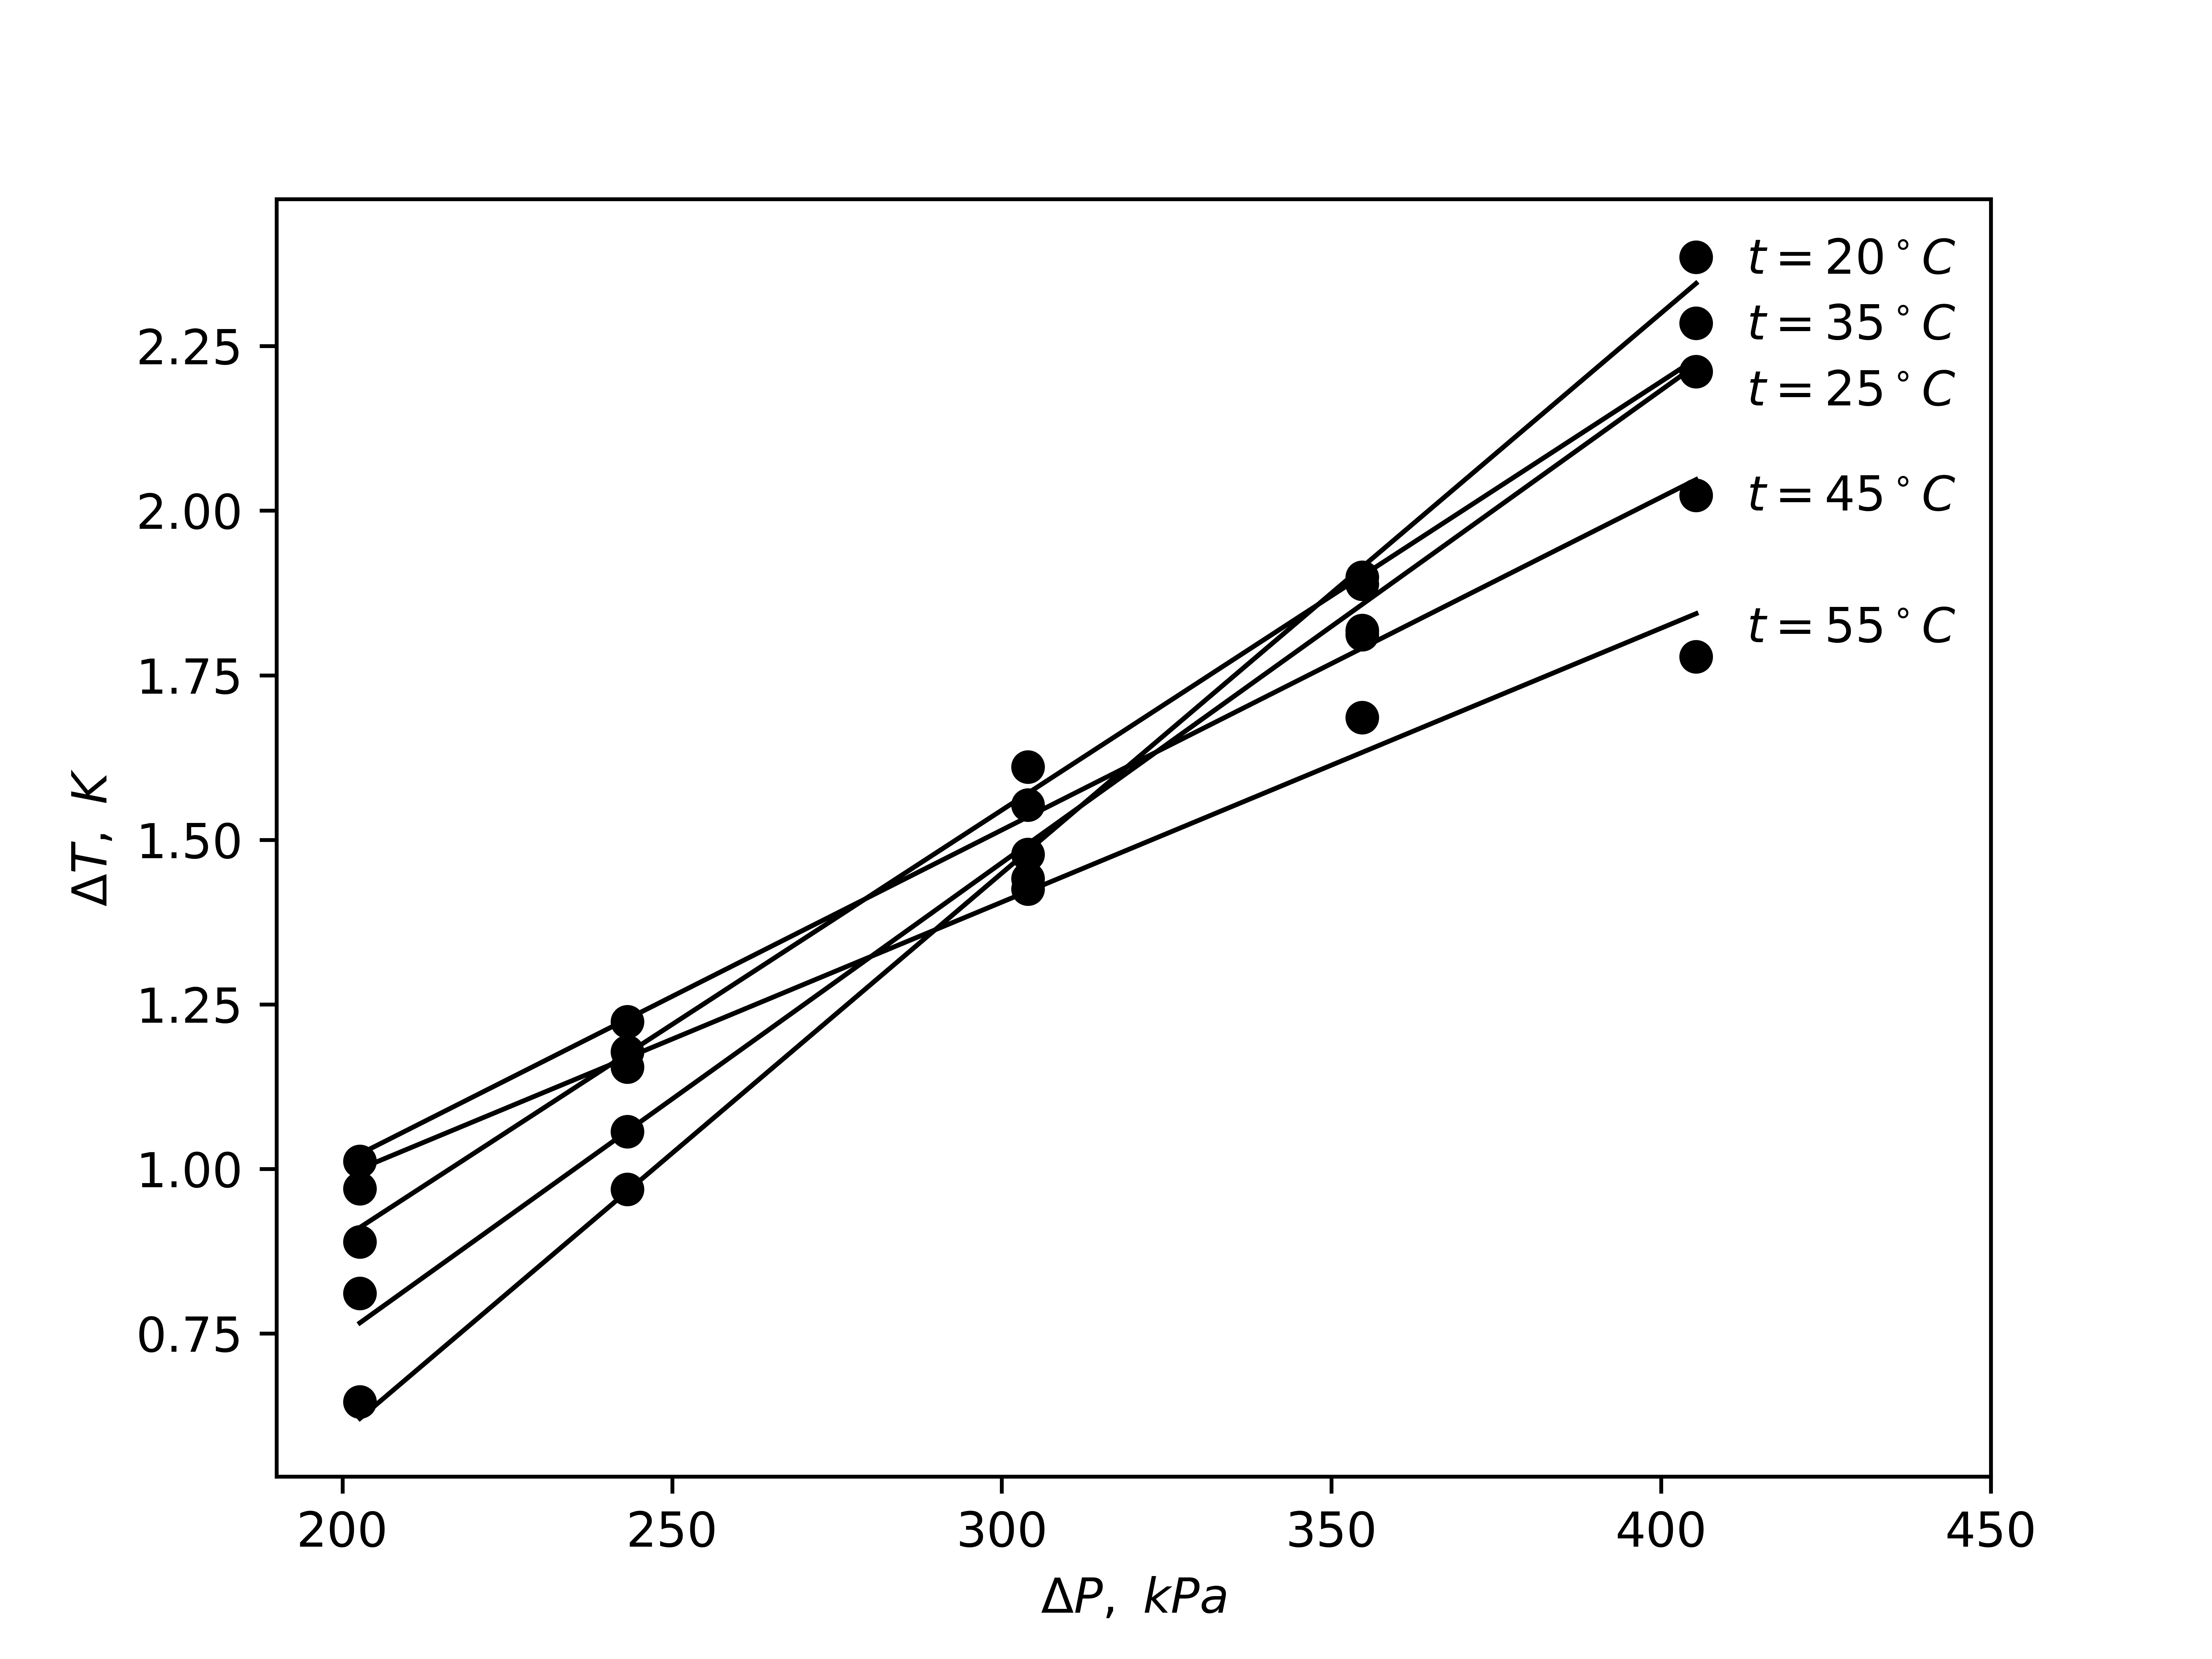
\includegraphics[scale=0.7]{terma_1_2.png}
\label{image1}
\caption{График зависимости $\Delta T(\Delta P)$ для различных температур}
\end{figure}

\begin{figure}[!ht]
\centering
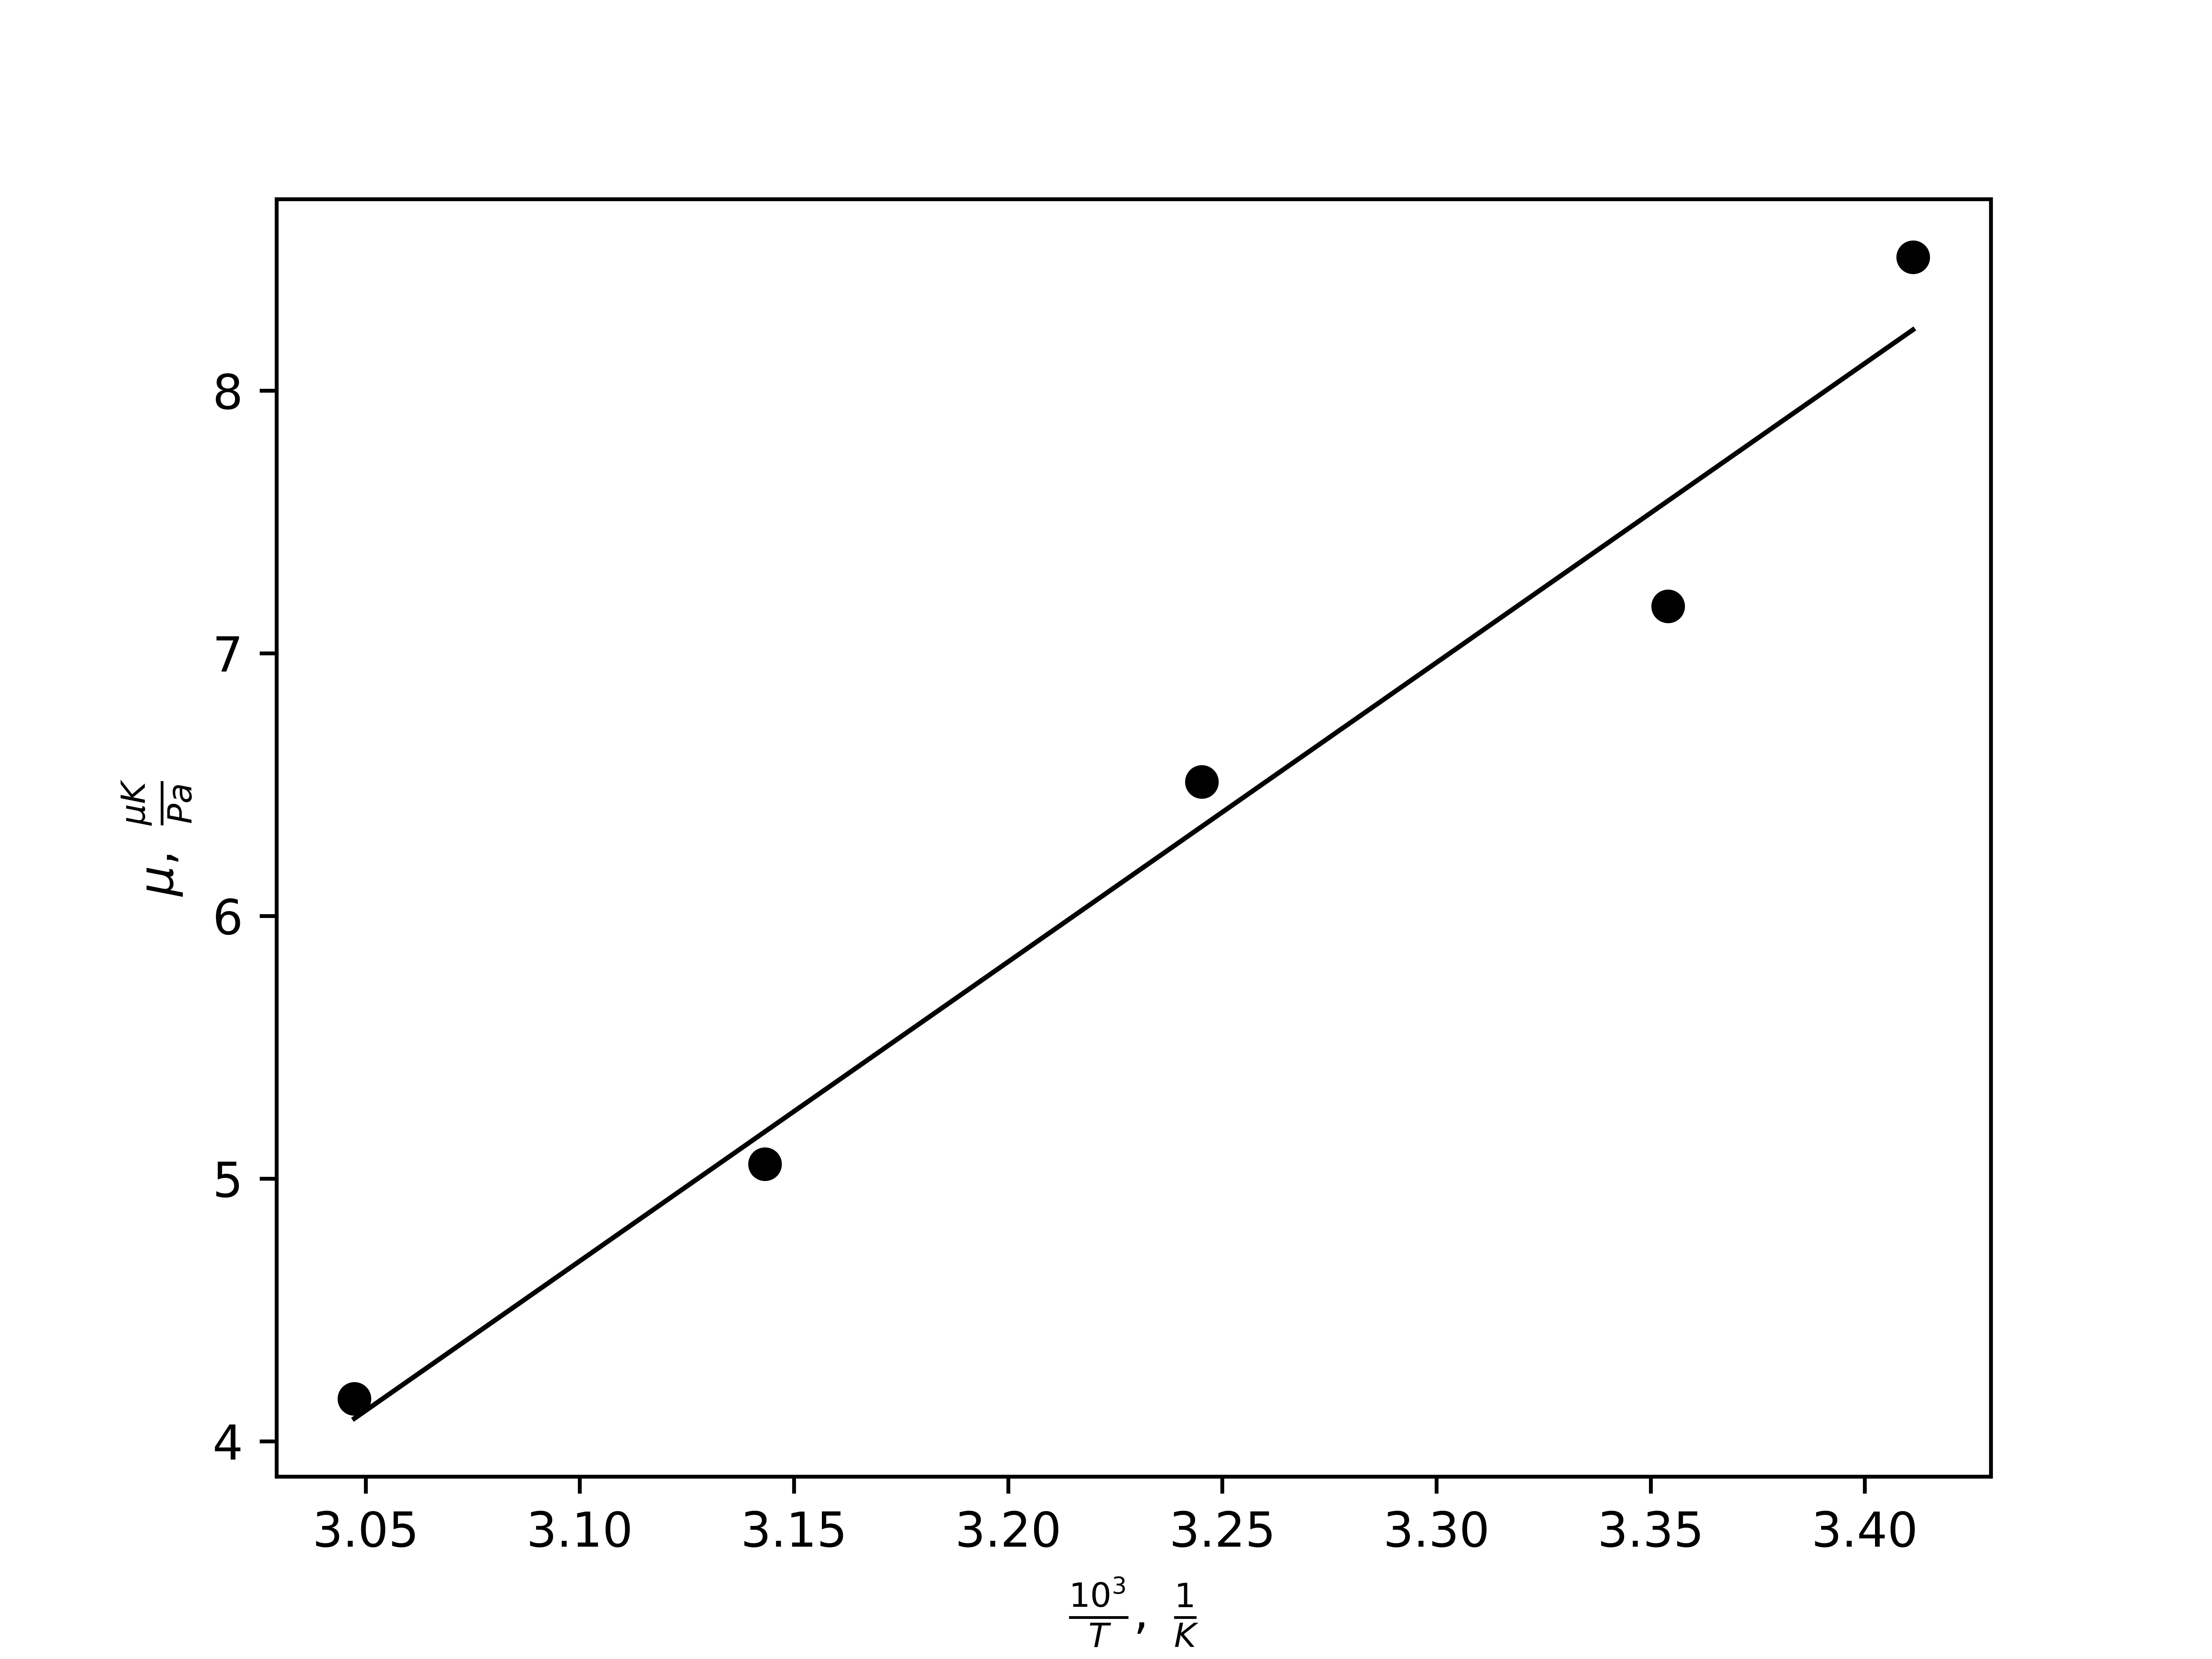
\includegraphics[scale=0.7]{terma_1_3.png}
\label{image2}
\caption{График зависимости $\mu(\frac{1}{T})$}
\end{figure}

\end{document}